\documentclass[11pt,letterpaper]{article}
\usepackage[top=3cm, bottom=2cm, left=2cm, right=2cm, columnsep=20pt]{geometry}
\usepackage{pdfpages}
\usepackage{graphicx}
\usepackage{etoolbox}
\apptocmd{\sloppy}{\hbadness 10000\relax}{}{}
% \usepackage[numbers]{natbib}
\usepackage[T1]{fontenc}
\usepackage{ragged2e}
\usepackage[french]{babel}
\usepackage{listings}
\usepackage{color}
\usepackage{soul}
\usepackage[utf8]{inputenc}
\usepackage[export]{adjustbox}
\usepackage{caption}
\usepackage{amsmath}
\usepackage{amssymb}
\usepackage{float}
\usepackage{csquotes}
\usepackage{fancyhdr}
\usepackage{wallpaper}
\usepackage{siunitx}
\usepackage[indent]{parskip}
\usepackage{textcomp}
\usepackage{gensymb}
\usepackage{multirow}
\usepackage[hidelinks]{hyperref}
\usepackage{abstract}
\renewcommand{\abstractnamefont}{\normalfont\bfseries}
\renewcommand{\abstracttextfont}{\normalfont\itshape}
\usepackage{titlesec}
\titleformat{\section}{\large\bfseries}{\thesection}{1em}{}
\titleformat{\subsection}{\normalsize\bfseries}{\thesubsection}{1em}{}
\titleformat{\subsubsection}{\normalsize\bfseries}{\thesubsubsection}{1em}{}

\usepackage{xcolor}
\definecolor{codegreen}{rgb}{0,0.6,0}
\definecolor{codegray}{rgb}{0.5,0.5,0.5}
\definecolor{codepurple}{rgb}{0.58,0,0.82}
\definecolor{backcolour}{rgb}{0.95,0.95,0.92}
\lstdefinestyle{mystyle}{
    backgroundcolor=\color{backcolour},   
    commentstyle=\color{codegreen},
    keywordstyle=\color{magenta},
    numberstyle=\tiny\color{codegray},
    stringstyle=\color{codepurple},
    basicstyle=\ttfamily\footnotesize,
    breakatwhitespace=false,         
    breaklines=true,                 
    captionpos=b,                    
    keepspaces=true,                 
    numbers=left,                    
    numbersep=5pt,                  
    showspaces=false,                
    showstringspaces=false,
    showtabs=false,                  
    tabsize=2
}
\lstset{style=mystyle}

\usepackage[most]{tcolorbox}
\newtcolorbox{note}[1][]{
  enhanced jigsaw,
  borderline west={2pt}{0pt}{black},
  sharp corners,
  boxrule=0pt, 
  fonttitle={\large\bfseries},
  coltitle={black},
  title={Note:\ },
  attach title to upper,
  #1
}

%----------------------------------------------------

\setlength{\parindent}{0pt}
\DeclareCaptionLabelFormat{mycaptionlabel}{#1 #2}
\captionsetup[figure]{labelsep=colon}
\captionsetup{labelformat=mycaptionlabel}
\captionsetup[figure]{name={Figure }}
\newcommand{\inlinecode}{\normalfont\texttt}
\usepackage{enumitem}
\setlist[itemize]{label=\textbullet}

\begin{document}
\begin{titlepage}
\center

\begin{figure}
    \ThisULCornerWallPaper{.4}{Polytechnique_signature-RGB-gauche_FR.png}
\end{figure}
\vspace*{2 cm}

\textsc{\Large \textbf{PHS2223 --} Introduction à l'optique moderne}\\[0.5cm]
\large{\textbf{Équipe : 04}}\\[1.5cm]

\rule{\linewidth}{0.5mm} \\[0.5cm]
\Large{\textbf{Expérience 2}} \\[0.2cm]
\text{Objectif de caméra}\\
\rule{\linewidth}{0.2mm} \\[2.3cm]

\large{\textbf{Présenté à}\\
  Guillaume Sheehy\\
  Esmat Zamani\\[2.5cm]
  \textbf{Par :}\\
  Émile \textbf{Guertin-Picard} (2208363)\\
  Laura-Li \textbf{Gilbert} (2204234)\\
  Tom \textbf{Dessauvages} (2133573)\\[3cm]}

\large{\today\\
Département de Génie Physique\\
Polytechnique Montréal\\}

\end{titlepage}

%----------------------------------------------------

\tableofcontents
\pagenumbering{roman}
\newpage

\pagestyle{fancy}
\setlength{\headheight}{14pt}
\renewcommand{\headrulewidth}{0pt}
\fancyfoot[R]{\thepage}

\pagestyle{fancy}
\fancyhf{}
\renewcommand{\headrulewidth}{1pt}
\fancyhead[L]{\textbf{PHS2223}}
\fancyhead[C]{Objectif de caméra : rapport final}
\fancyhead[R]{\today}
\fancyfoot[R]{\thepage}

\pagenumbering{arabic}
\setcounter{page}{1}

%----------------------------------------------------

\section{Résultats}

Cette section présente et analyse les différentes images capturées lors des
manipulations.

\subsection{Profondeur de champ}

Tout d'abord, les images qui suivent permettent d'analyser la profondeur de champ
du système de lentilles dans deux configurations, soit celle offrant un zoom minimal,
et celle offrant un zoom maximal. Pour obtenir ces images, à chaque extrême de zoom,
le focus est mis sur une cible graduée, à une distance de 1m. Ensuite, cette cible est
déplacée d'abord devant, puis derrière la distance focale, jusqu'à perte du focus.
Cela est déterminé approximativement par la perte de définition entre les graduations
présentes sur la cible. La distance de déplacement jusqu'à cette perte est notée afin
de faire le calcul de profondeur de champ. Pour le zoom minimal :

\begin{figure}[H]
  \centering
  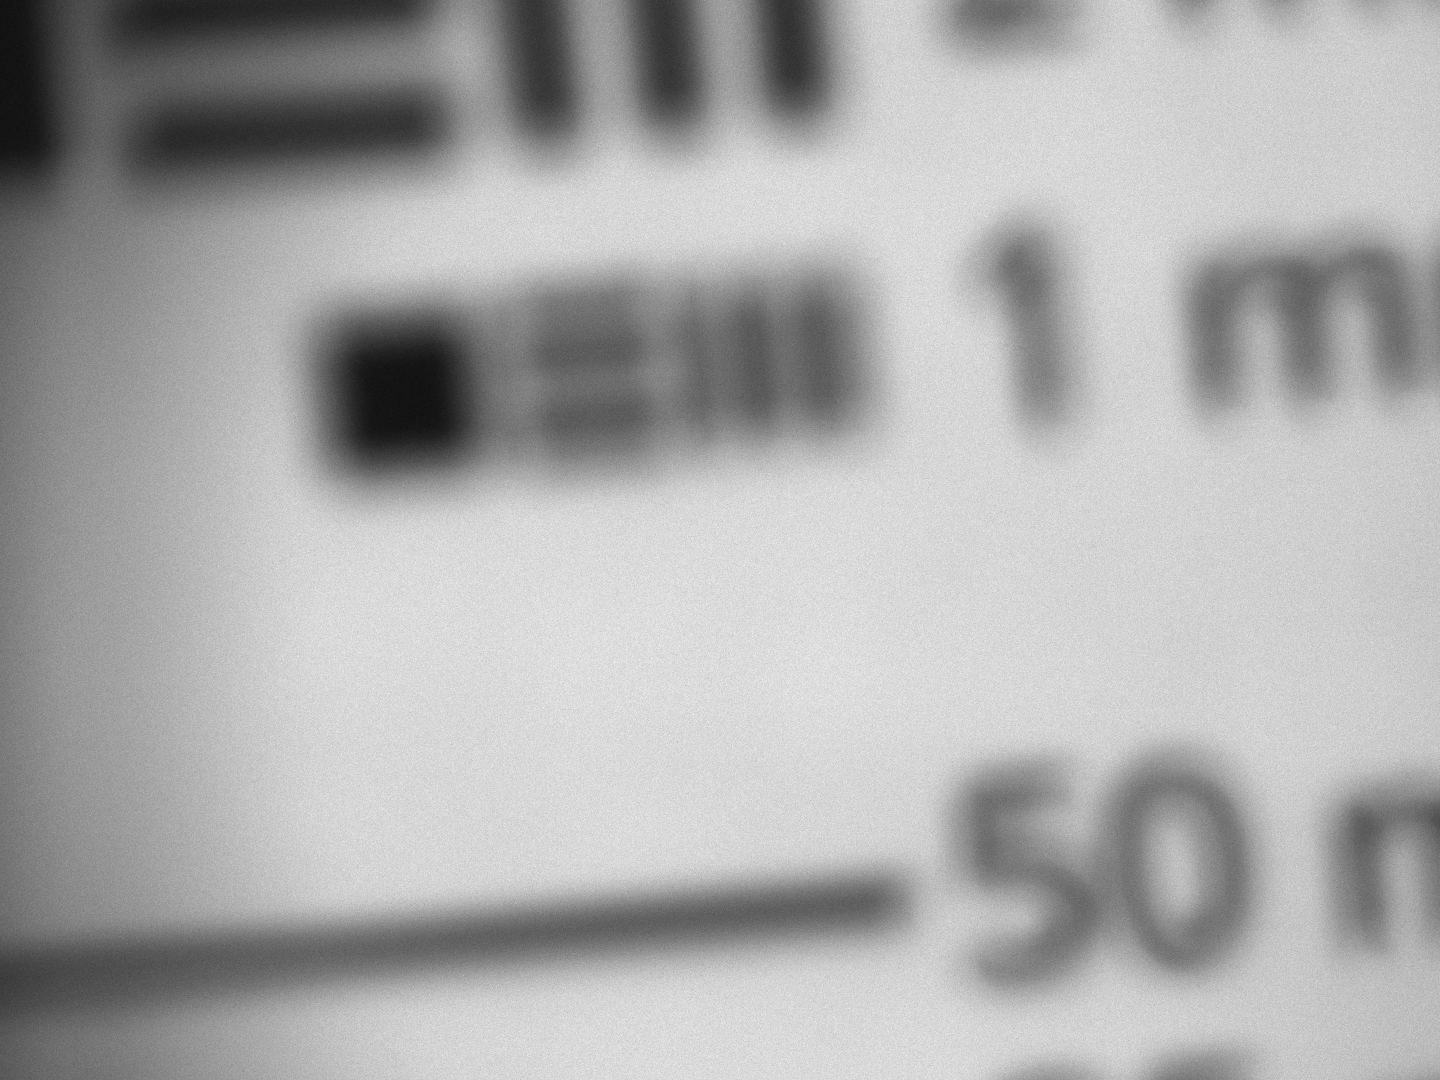
\includegraphics[scale=0.3]{prof_0.458m_min.png}
  \caption{Photo du perte de focus en amont du point focal de 1m, soit à 0.458m,
  pour le zoom minimal.}
  \label{prof_avant_min}
\end{figure}

\begin{figure}[H]
  \centering
  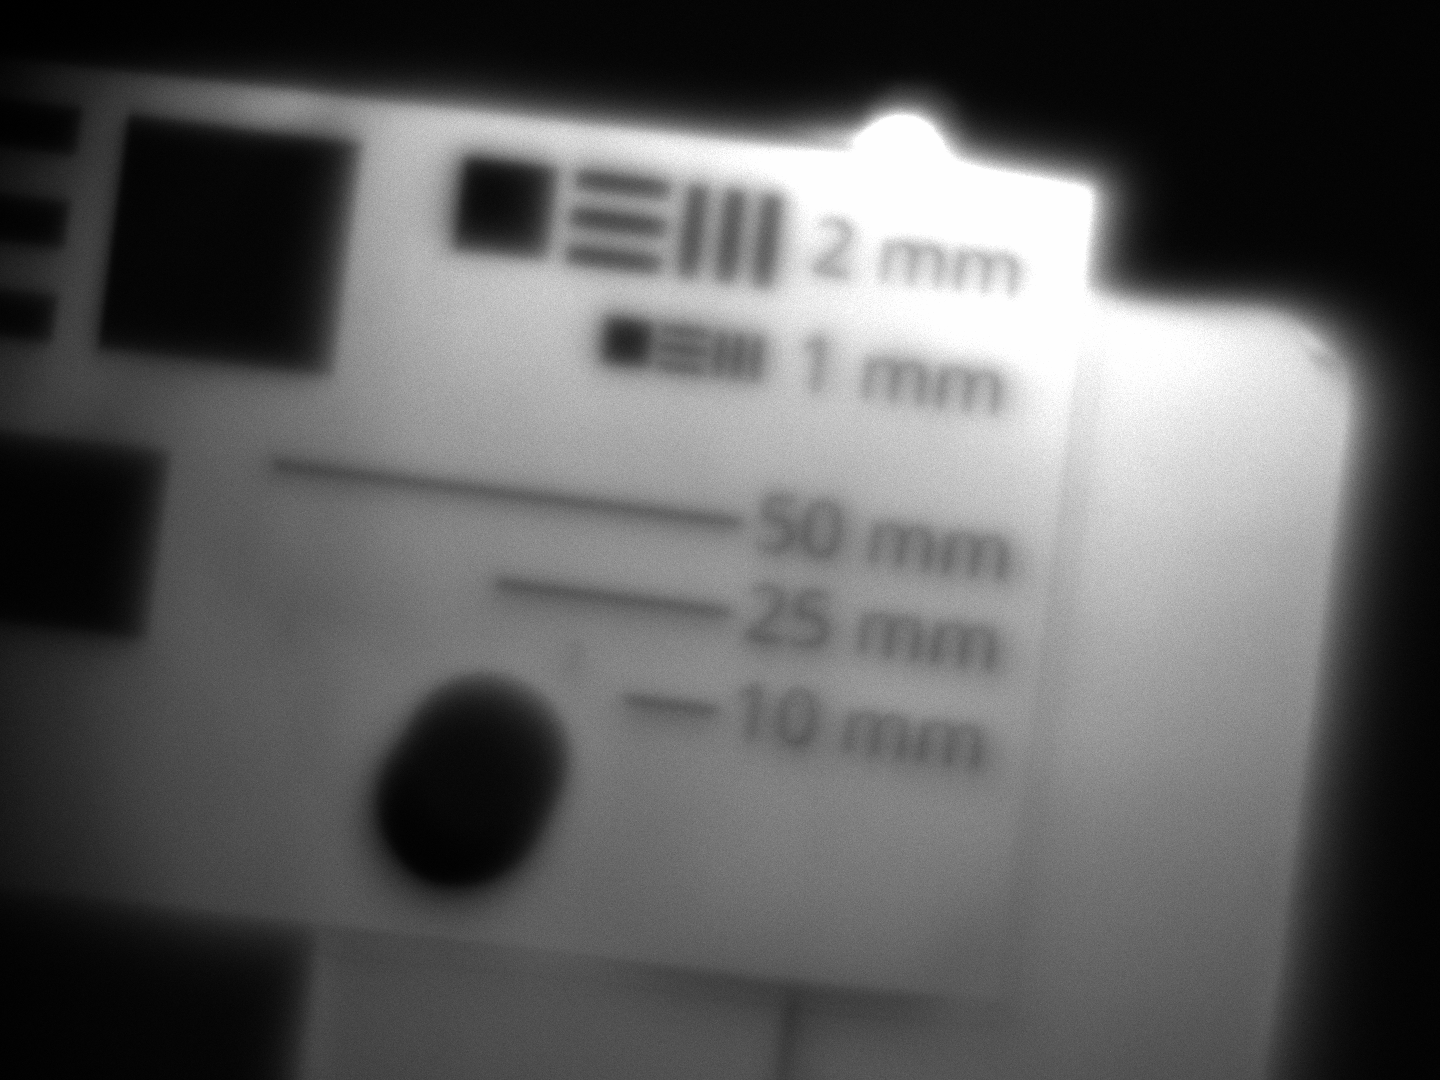
\includegraphics[scale=0.3]{prof_1.986_min.png}
  \caption{Photo du perte de focus en aval du point focal de 1m, soit à 1.986m,
  pour le zoom minimal.}
  \label{prof_arr_min}
\end{figure}

La différence entre les deux positions de perte de focus est donc la profondeur de
champ. Il est donc possible de trouver $\delta_{z,min}= 1.528$m. Pour le zoom maximal :

\begin{figure}[H]
  \centering
  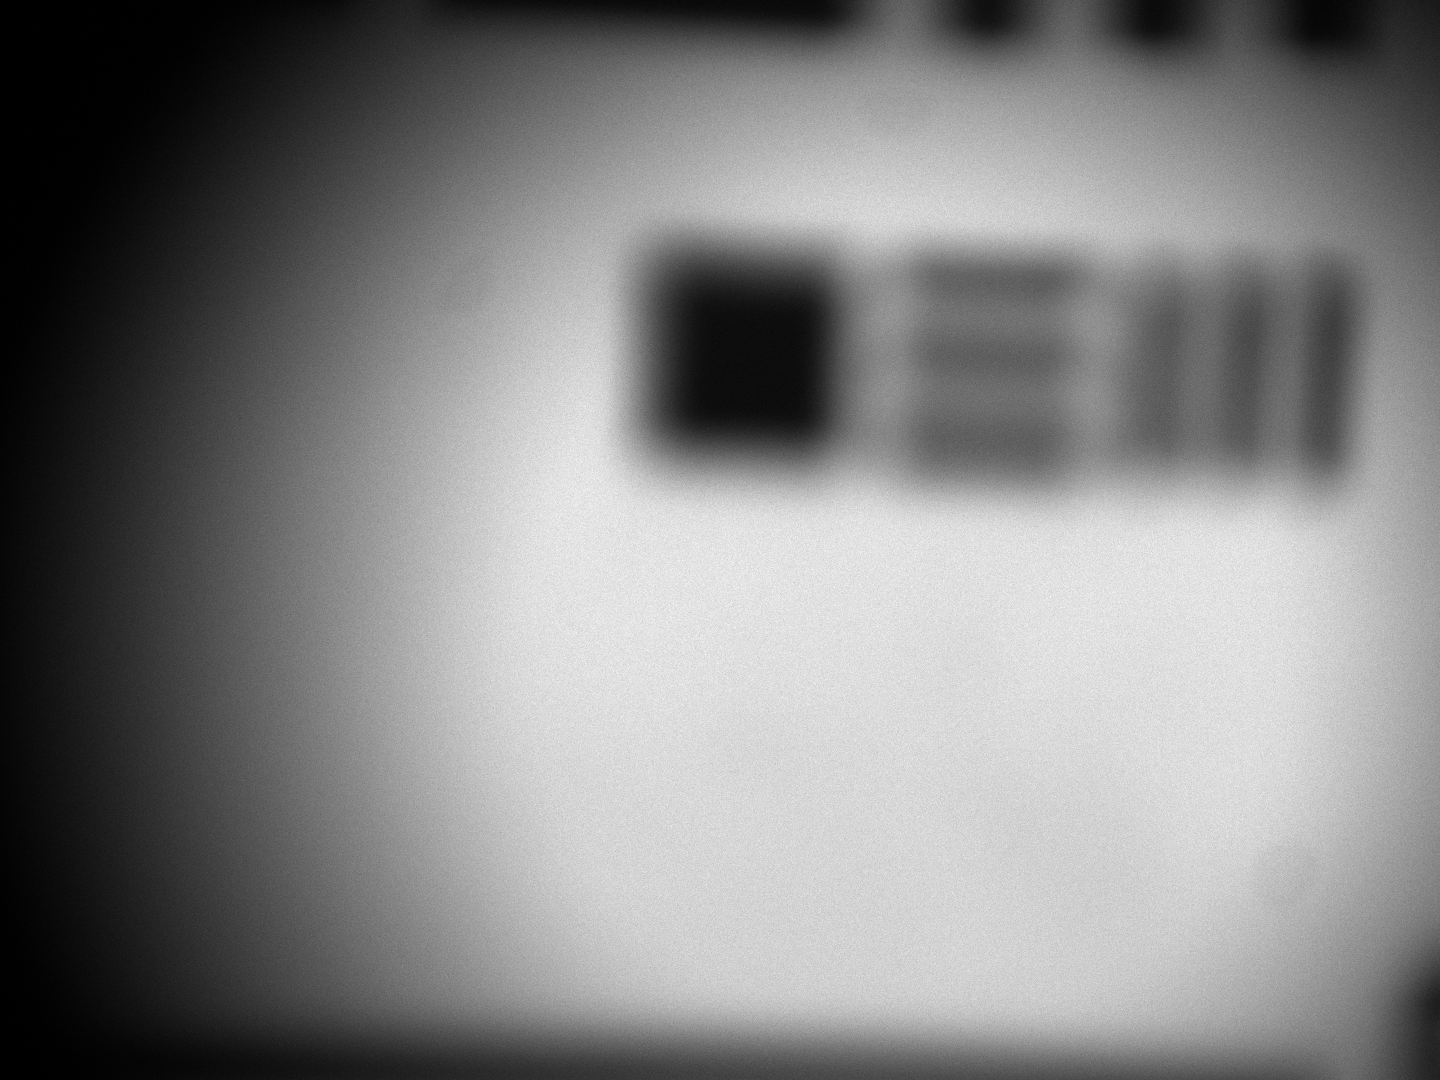
\includegraphics[scale=0.3]{prof_0.711m_max.png}
  \caption{Photo du perte de focus en amont du point focal de 1m, soit à 0.711m,
  pour le zoom maximal.}
  \label{prof_avant_max}
\end{figure}

\begin{figure}[H]
  \centering
  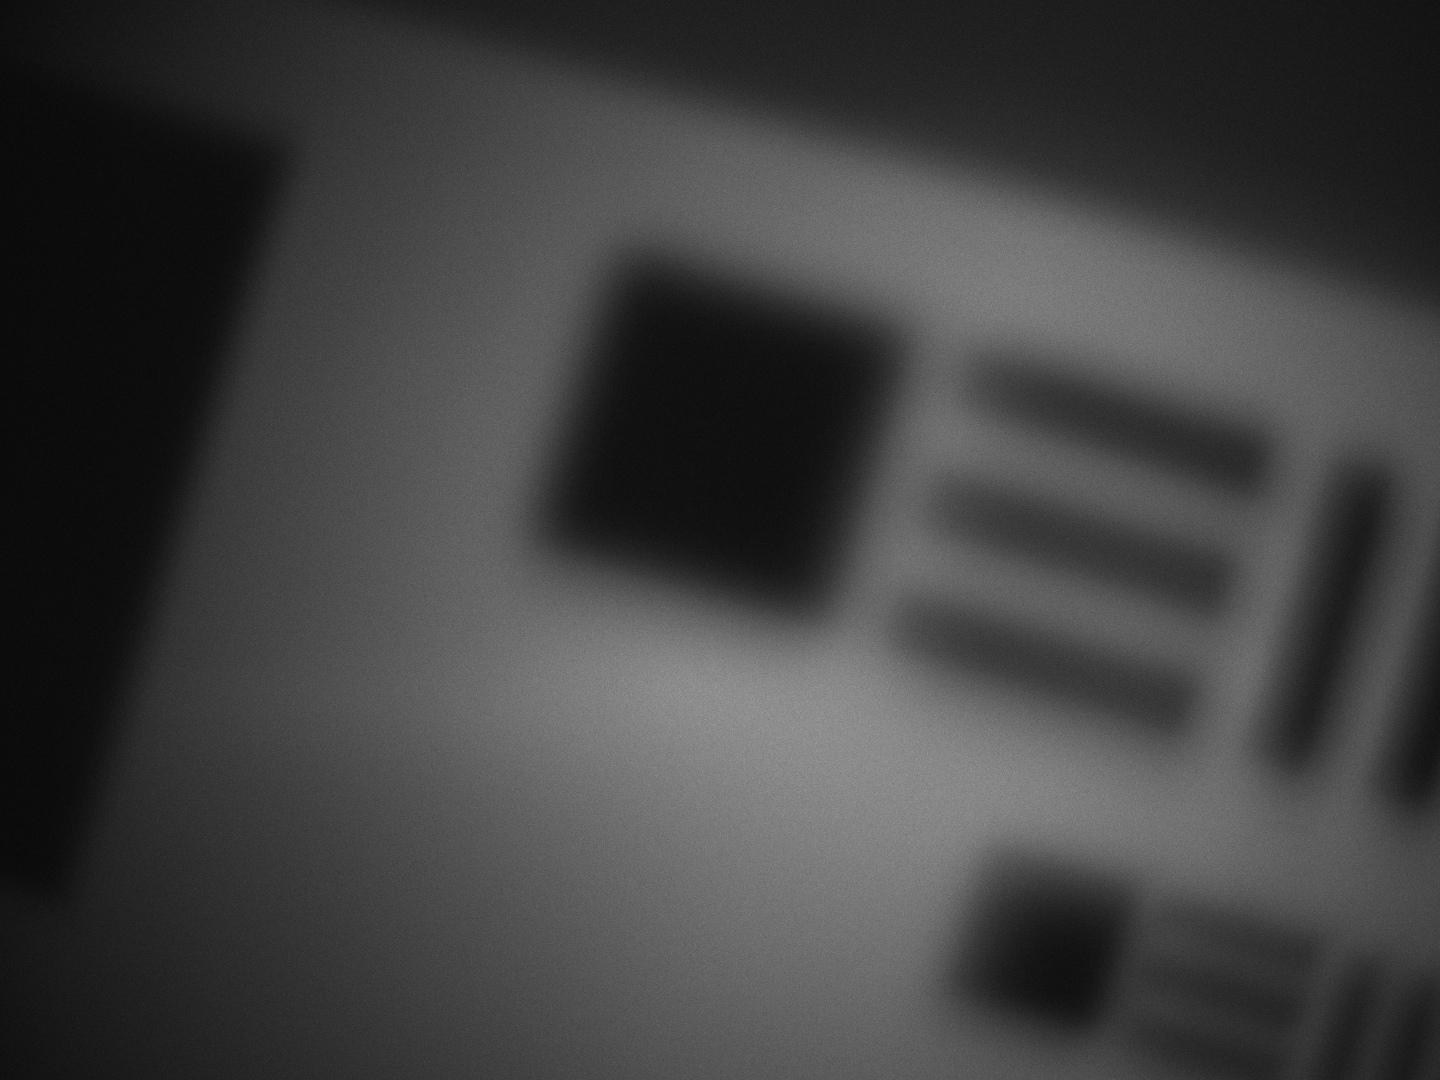
\includegraphics[scale=0.3]{prof_1.174_max.png}
  \caption{Photo du perte de focus en aval du point focal de 1m, soit à 1.174m,
  pour le zoom maximal.}
  \label{prof_arr_max}
\end{figure}

De la même manière, il est possible de trouver la profondeur de champ 
$\delta_{z,max}= 0.463$m.


\subsection{Analyse de résolution}
 
Afin d'analyser la résolution de la caméra, deux photos de la cible ont été prises
au focus de la caméra à 1m, autant pour le zoom minimal que pour le zoom maximal : 

\begin{figure}[h!]
    \centering
    \begin{minipage}[t]{0.47\linewidth}
        \centering
        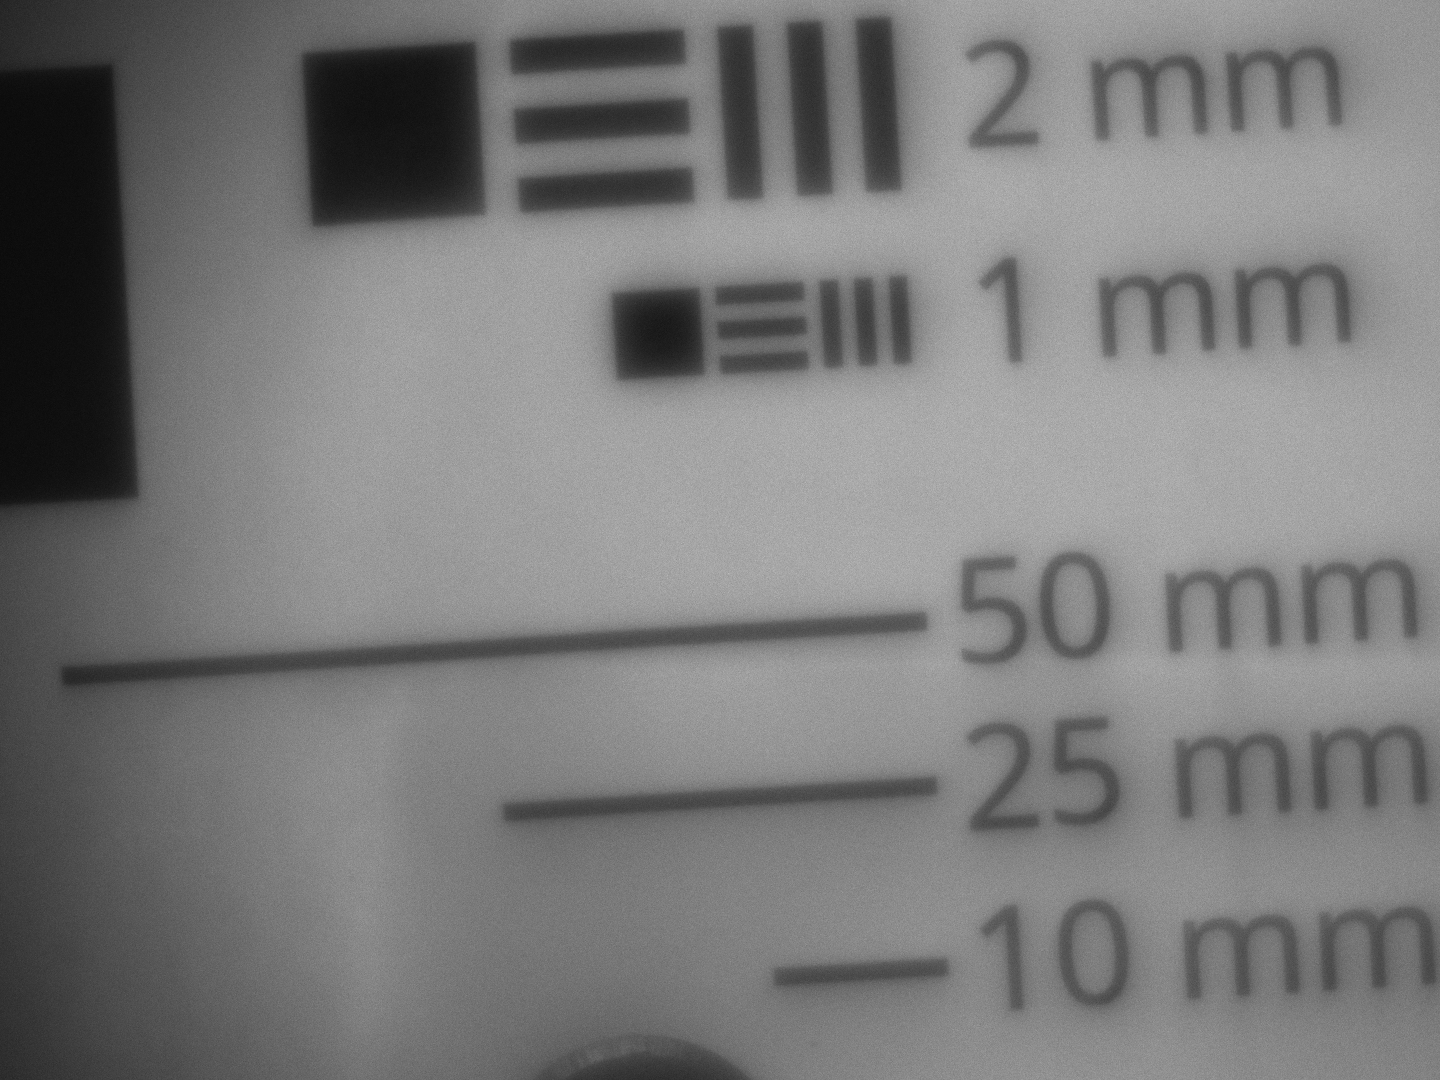
\includegraphics[scale=0.22]{res_1m_min.png}
        \caption{Photo de l'objet au focus de 1m pour le zoom minimal.}
        \label{res_min}
    \end{minipage}\hfill
    \begin{minipage}[t]{0.5\linewidth}
        \centering
        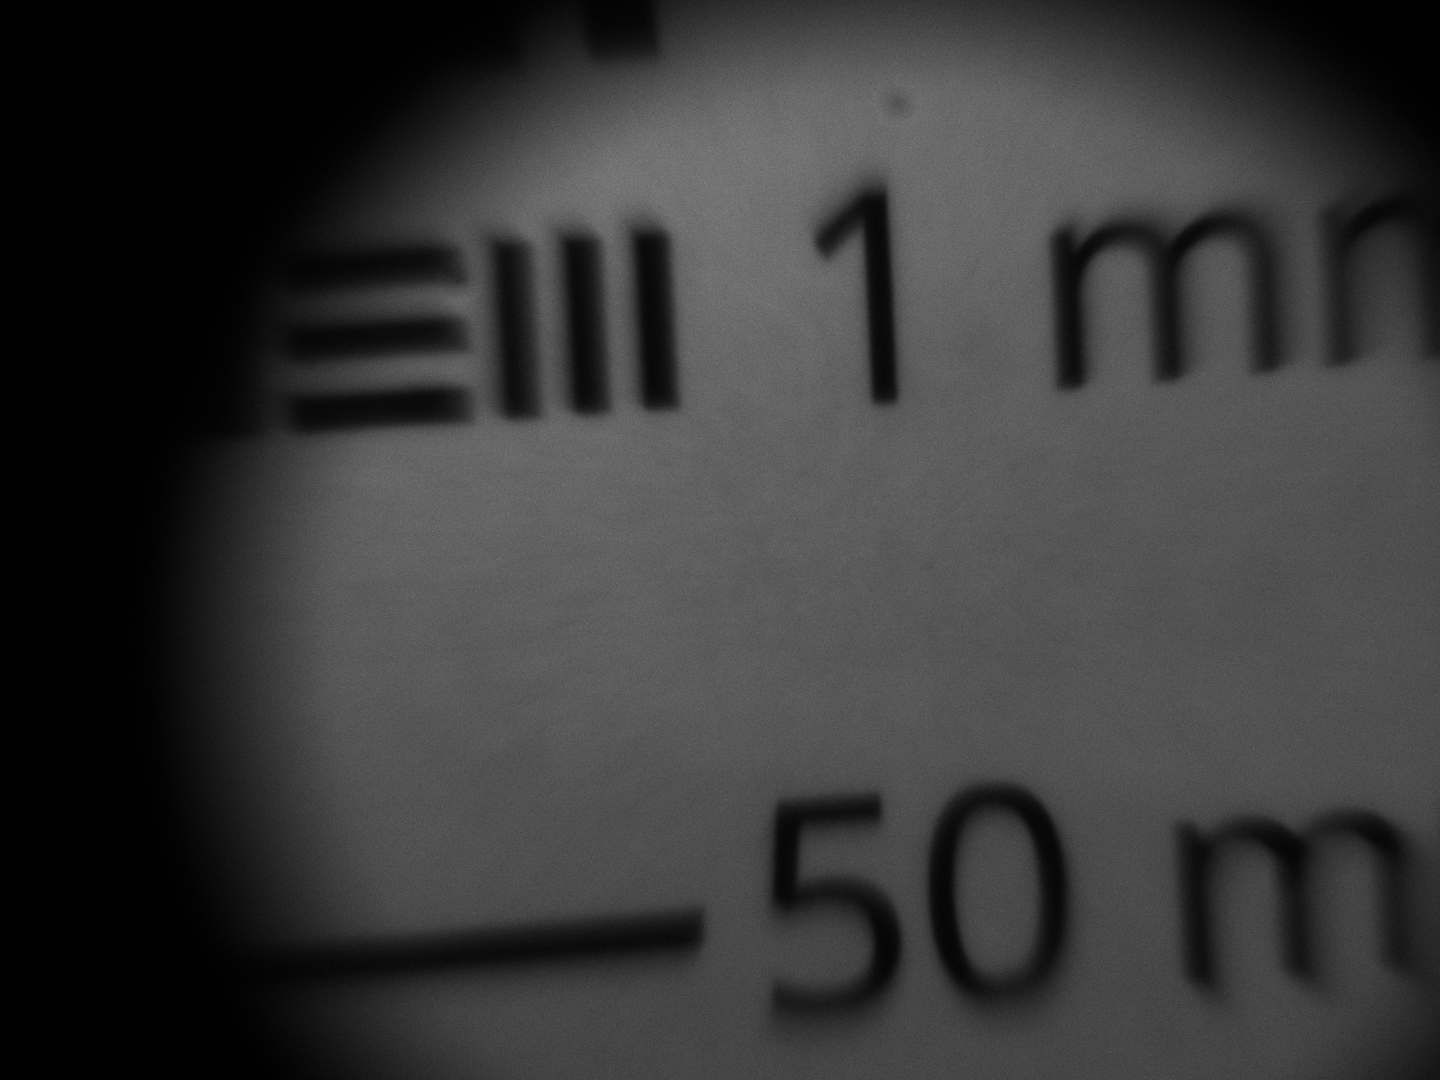
\includegraphics[scale=0.22]{res_1m_max.png}
        \caption{Photo de l'objet au focus de 1m pour le zoom maximal.}
        \label{res_max}
    \end{minipage}
\end{figure}

La résolution de ces images peut être définie de façon générale comme étant : 

\begin{equation}
    r = \frac{taille \: de \: r\textit{é}f\textit{é}rence}{nombre \: de \: pixels} \: [L\cdot pixels^{-1}]
    \label{r}
\end{equation}

La taille de référence correspond à une dimension connue de l'espace réel. Sur les figures \ref{res_min} et \ref{res_max} elle est représentée par les barres de dimensions fixe : 1 mm, 2 mm, 10 mm, 25 mm et 50 mm. Pour se ramener à l'équation \ref{r} il est donc nécessaire de comptabiliser le nombre de pixels occupé par chacune de ces tiges, ce qui est possible grâce à un programme python, disponible en annexe. Les figures \ref{detec_min} et \ref{detec_max} présente les contours détectés pour chacune des images présentées en figure \ref{res_min} et \ref{res_max}

\begin{figure}[h!]
    \centering
    \begin{minipage}[t]{0.46\linewidth}
        \centering
        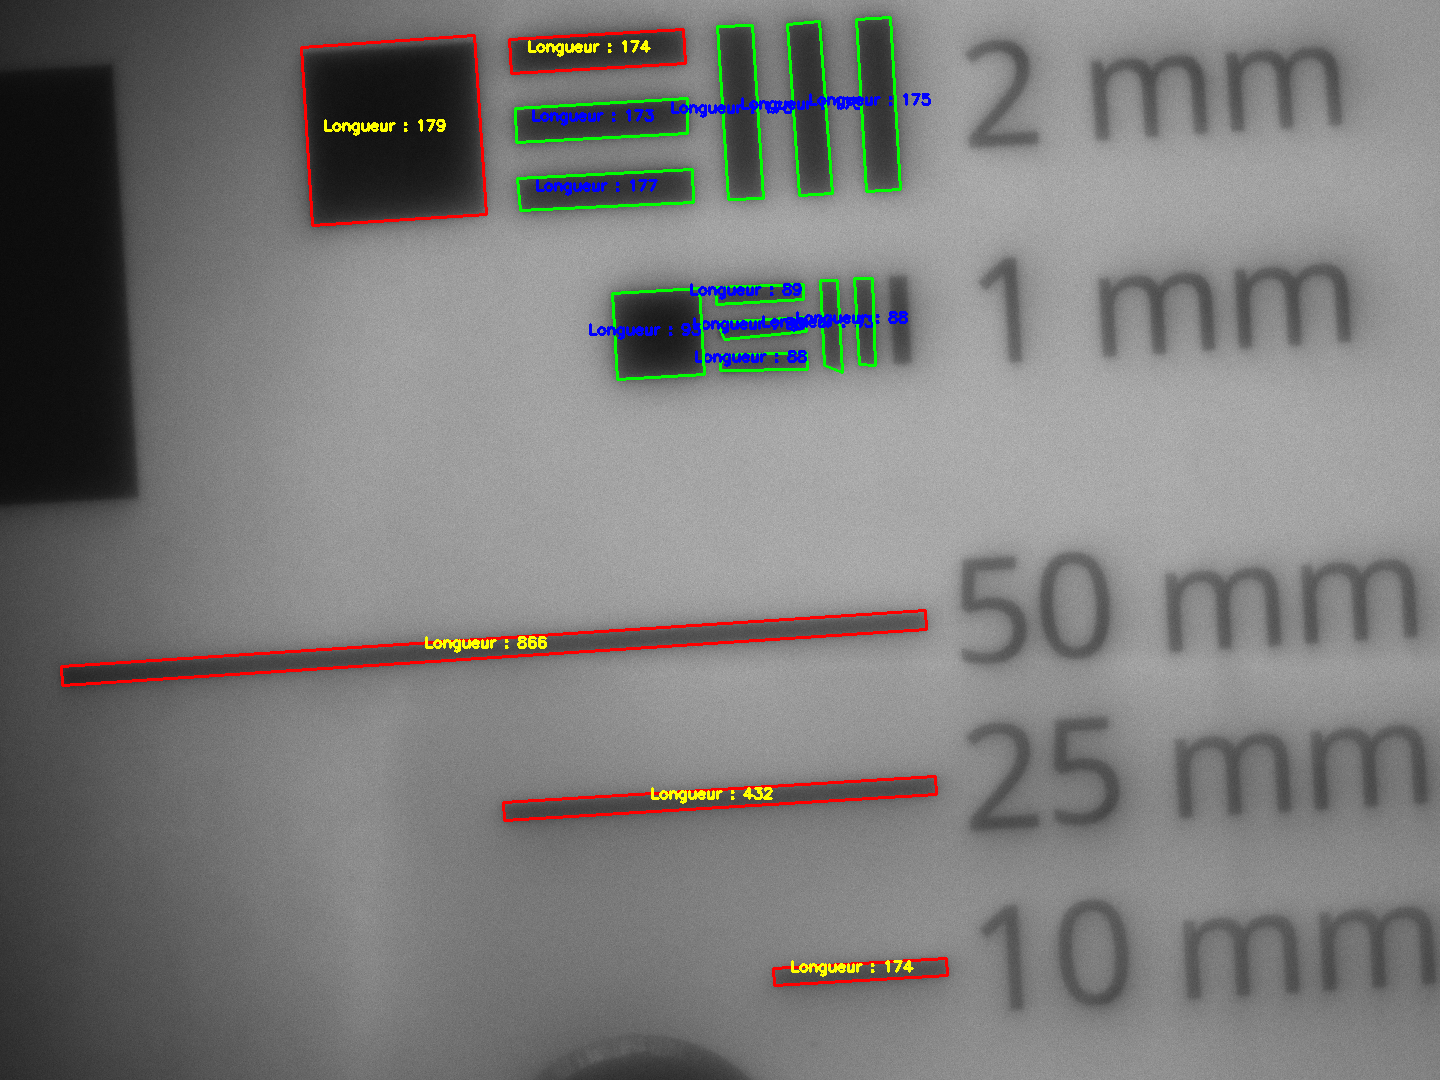
\includegraphics[scale=0.17]{rectangles_detectes_min.png}
        \caption{Contours obtenus sur les tiges de références le zoom minimal.}
        \label{detec_min}
    \end{minipage}\hfill
    \begin{minipage}[t]{0.48\linewidth}
        \centering
        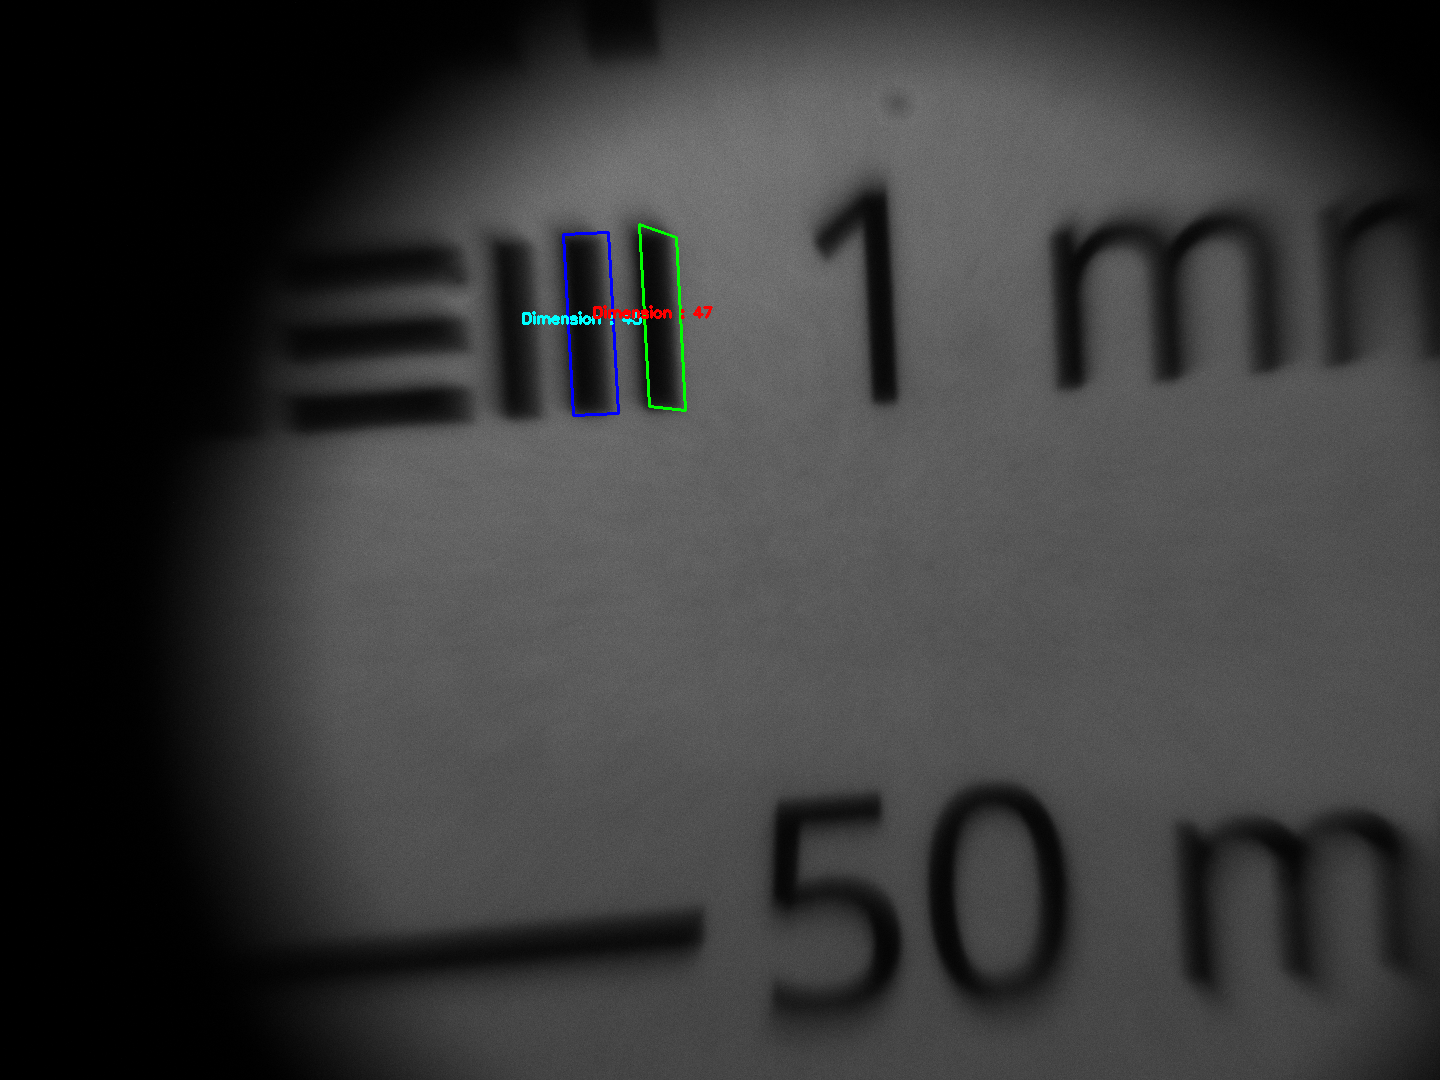
\includegraphics[scale=0.17]{rectangles_detectes_max.png}
        \caption{Contours obtenus sur les tiges de références le zoom maximal.}
        \label{detec_max}
    \end{minipage}
\end{figure}

Les données "dimensions" représentées en pixels ont été répertoriées dans des tableaux

\begin{table}[h!]
\centering
\scalebox{1}{ % Ajustez le facteur de mise à l'échelle ici (0.8 par exemple)
\begin{tabular}{|l|l|l|l|}
\hline
\textbf{Taille réelle (mm)} & \textbf{Nombre d'échantillons} & \textbf{Moyenne (pixels)} & \textbf{Écart-type (pixels)} \\ \hline
1                           & 6 &  21.500000                & 1.516575                     \\ \hline
2                           & 6 & 43.222657                & 4.664085                     \\ \hline
10                          & 1 & 174.214767               & 0.000000                     \\ \hline
25                          & 1 & 432.901978               & 0.000000                     \\ \hline
50                          & 1 & 866.068909               & 0.000000                     \\ \hline
\end{tabular}%
}
\caption{Tableau du nombre de pixels en fonction des tiges de référence pour le zoom minimum.}
\label{tige_min}
\end{table}

\begin{table}[h!]
\centering
\scalebox{1}{ % Ajustez le facteur de mise à l'échelle ici (0.8 par exemple)
\begin{tabular}{|l|l|l|l|}
\hline
\textbf{Taille réelle (mm)} & \textbf{Nombre d'échantillons} & \textbf{Moyenne (pixels)} & \textbf{Écart-type (pixels)} \\ \hline
1                           & 2 & 46.048563                 & 1.345535                    \\ \hline
\end{tabular}%
}
\caption{Tableau du nombre de pixels en fonction des tiges de référence pour le zoom maximum.}
\label{tige_max}


\end{table}

Dans ces tableaux les données ont été traitées de façons statistiques en fonction du nombre d'échantillons et de leur valeur. En les mettant ensuite en lien avec l'équation \ref{r} il est possible d'en déduire des valeurs de résolution. Le tableau \ref{table_res} présente les résolutions obtenues en fonction des positions de zoom. 

\begin{table}[h!]
\centering
\scalebox{1}{ % Ajustez le facteur de mise à l'échelle ici (0.8 par exemple)
\begin{tabular}{|l|l|l|}
\hline
\textbf{Zoom} & \textbf{Résolution (mm/pixel)} & \textbf{Écart-type (résolution)} \\ \hline
Min                           & 0.053133               & 0.006156                    \\ \hline
Max                           & 0.021716                 & 0.000000                    \\ \hline
\end{tabular}%
}
\caption{Tableau de la résolution en fonction de la position du zoom.}
\label{max_patron}
\end{table}

Les statistiques présentées dans ce tableaux n'ont pas été mise directement en relation avec celle des tableaux \ref{tige_min} et \ref{tige_max}, elles ne représentent que celles obtenues grâce au calcul des résolutions pour les différentes tiges de référence. Ces résultats sont très proches de ceux obtenus de façon théorique dans le rapport préliminaire malgré un facteur d'échelle non explicité sur les graphiques du rapport préliminaire. Le tableau \ref{écart} présente les écarts entre les valeurs théoriques et expérimentales. 

\begin{table}[h!]
\centering
\scalebox{1}{ % Ajustez le facteur de mise à l'échelle ici (0.8 par exemple)
\begin{tabular}{|l|l|l|}
\hline
\textbf{Résolution théorique} & \textbf{Résolution expérimentale} & \textbf{Écart (absolu)} \\ \hline
0.050                           & 0.053133               & 0.003                   \\ \hline
0.023 \textbf{(A VERIFIER)}               & 0.021716                 & 0.001                   \\ \hline
\end{tabular}%
}
\caption{Tableau des écarts entre les valeurs théoriques et expérimentales.}
\label{écart}
\end{table}


\subsection{Vignettage}

L'analyse du vignettage se fait qualitativement en comparant sa présence aux deux
niveaux de zoom, mais aussi à deux positions de l'objet, soit 1m et "l'infini". 
Un vignettage fort est défini par un contour net entre une région circulaire de 
l'image et la région "extérieure" au cercle comme noir. Moins ce contour est net, 
moins le vignettage est fort. Pour l'objet à 1m, en commencant par le zoom minimal : 

\begin{figure}[H]
  \centering
  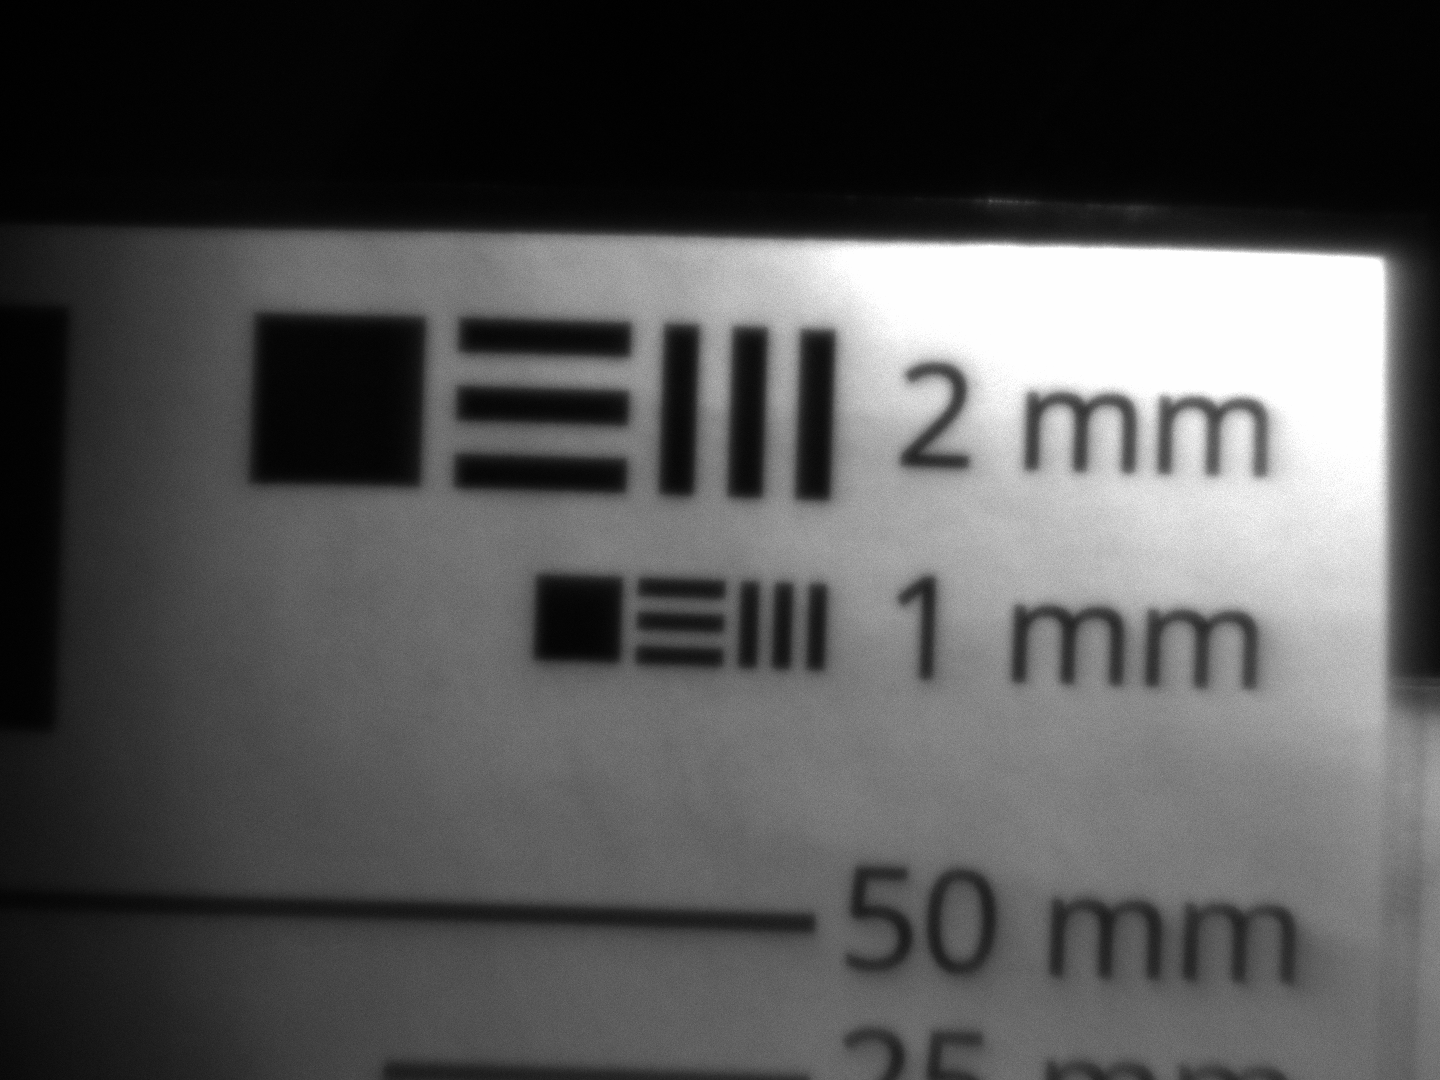
\includegraphics[scale=0.3]{vig_1m_min.png}
  \caption{Image avec vignettage pour un objet à 1m vu avec un zoom minimal.}
  \label{vig_m_min}
\end{figure}

Ce vignettage peut être considéré comme modéré en regardand la région assombrie en 
bas à gauche. Ensuite, avec le zoom maximal :

\begin{figure}[H]
  \centering
  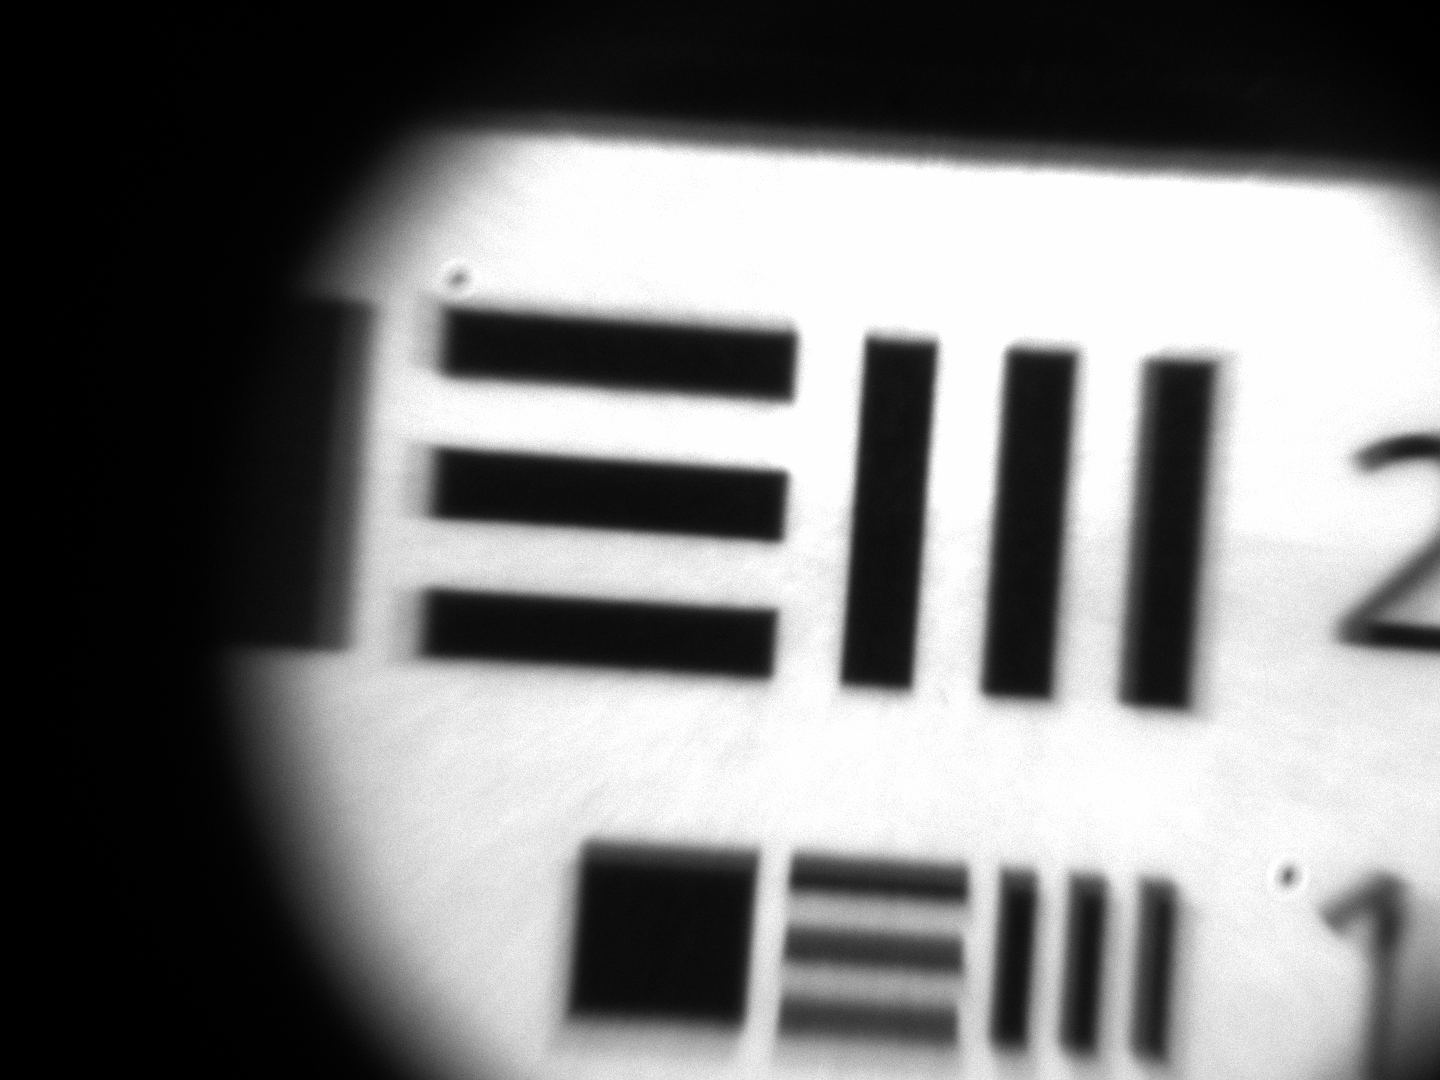
\includegraphics[scale=0.3]{vig_1m_max.png}
  \caption{Image avec vignettage pour un objet à 1m vu avec un zoom maximal.}
  \label{vig_m_max}
\end{figure}

Le vignettage est beaucoup plus important avec ce niveau de zoom, tel que montré par
par la région totalement sombre à gauche. Pour l'objet à l'infini avec le zoom minimal :

\begin{figure}[H]
  \centering
  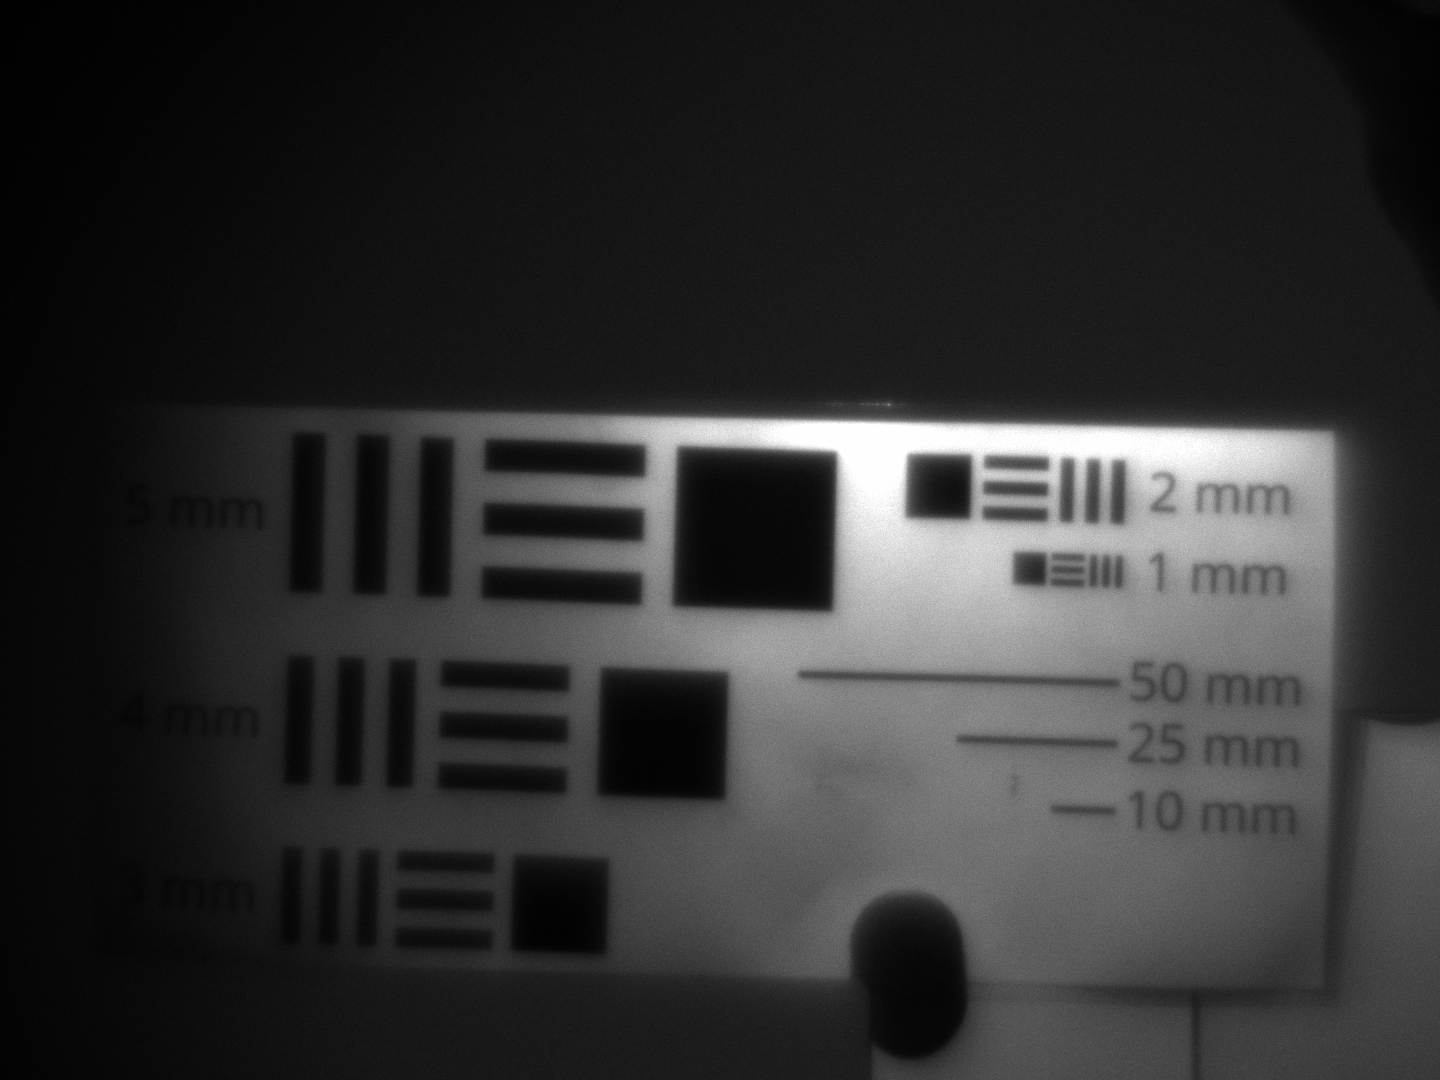
\includegraphics[scale=0.3]{vig_inf_min.png}
  \caption{Image avec vignettage pour un objet à l'infini vu avec un zoom minimal.}
  \label{vig_inf_min}
\end{figure}

Ce vignettage est faible, mais percevable à chaque coin inférieur de l'image. Avec
le zoom maximal :

\begin{figure}[H]
  \centering
  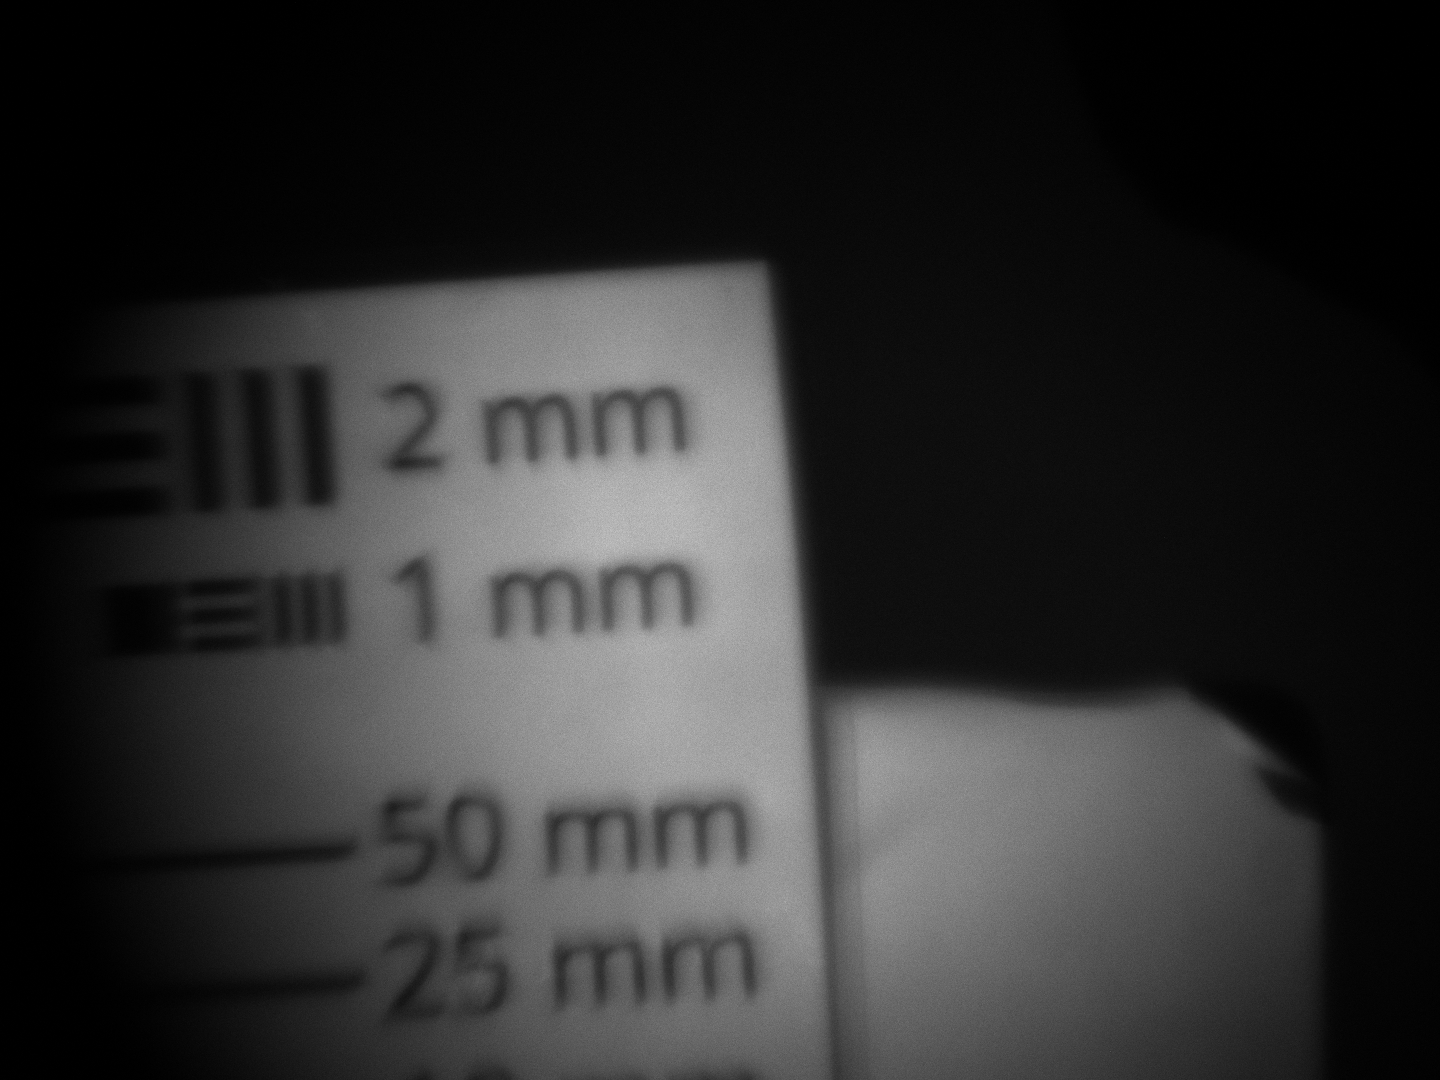
\includegraphics[scale=0.3]{vig_inf_max.png}
  \caption{Image avec vignettage pour un objet à l'infini vu avec un zoom maximal.}
  \label{vig_inf_max}
\end{figure}

Enfin, ce vignettage est aussi modéré, voir fort. On voit une grande région 
assombrie à gauche, mais moins définie qu'à la figure \ref{vig_m_max}.

\subsection{Facteur de zoom}
\textcolor{red}{[TODO Tom]} 
% TODO par Tom : Utiliser les tailles physiques des pixels pour voir la taille de
% la cible a grossi de quel facteur

\subsection{Tableau des caractéristiques}

\begin{table}[h]
\centering
\begin{tabular}{|l|l||l|l|l||c|}
\hline
\textbf{Distance objet} & \textbf{Zoom} & \textbf{Profondeur champ} & \textbf{Résolution} & \textbf{Vignettage} & \textbf{Facteur zoom} \\ \hline
1m & min  & 1.528m & \textcolor{red}{[valeur]} & modéré & \multirow{4}{*}{g} \\ \cline{1-5}
1m & max  & 0.463m & \textcolor{red}{[valeur]} & très fort & \\ \cline{1-5}
Infini & min  & - & \textcolor{red}{[valeur]} & faible & \\ \cline{1-5}
Infini & max  & - & \textcolor{red}{[valeur]} & fort & \\ \hline
\end{tabular}
\caption{Tableau des principaux résultats acquis lors des manipulations.}
\end{table}


\section{Discussion}

Cette section est dédiée à l'analyse, l'interprétation et la critique des résultats
obtenus lors des manipulations.

\subsection{Retour sur l'hypothèse}

Les hypothèses émises précédemment comparaient certaines caractéristiques de performance
de la caméra à la distance entre les lentilles $L_2$ et $L_1$. Cela revient 
essentiellement à analyser les caractéristiques en fonction du zoom. En guise de rappel,
les hypothèses suivantes ont été émises :

\begin{itemize}
\item La profondeur de champ reste constante à environ 6.6mm peu importe le zoom.
\item Plus l'espace entre les lentilles est élevé, plus le zoom est important.
\item Plus l'espace entre les lentilles est élevé, moins la résolution est importante.
\end{itemize}

D'abord, il est très facile de voir que la première hypothèse sur la profondeur
de champ est fausse. Non seulement le comportement n'était pas constant avec le zoom,
mais l'ordre de grandeur est en réalité plus près du mètre que du millimètre. Cette
disparité s'explique facilement par l'omission de l'iris ajustable dans la simulation
faite sur python. Cette dernière peut jouer le rôle d'ouverture d'arrêt, et donc avoir
un impact direct sur la profondeur de champ \textcolor{red}{Source A}. Sans l'avoir 
prise en considération, il est normal que l'hypothèse soit erronée.

% Source A : ndc L8-s5

Ensuite, il est possible de confirmer la deuxième hypothèse sur le zoom. La
configuration avec le zoom maximal utilisé lors de la prise de photo était celle avec
la plus grande séparation entre les lentilles. Le comportement précis de la courbe
trouvée par simulation ne peut être confirmé toutefois, car seulement les deux extrêmes
de zoom ont été testés. Cela implique donc qu'une augmentation de la distance $L_1 - L_2$ implique une augmentation du zoom.

Cette dernière conclusion aide à redéfinir la troisième hypothèse : plus le zoom est
grand, moins la résolution est importante. \textcolor{red}{A FINIR : Emile}.

\subsection{Sources d'erreurs}
Les divergences des résultats par rapport aux hypothèses émises peuvent être expliquées par certaines causes d'erreurs. Une première cause possible correspond à l'éclairage inconstant de la pièce. Ces fluctuations, causées par l'ouverture et la fermeture de lumières, ont influencé les conditions d'illumination des objets photographiés, notamment en affectant l'exposition, le contraste et la netteté de l'image. Ensuite, lorsque la profondeur de champ a été observée, certaines des photos prises impliquaient de se tenir entre deux tables. Pour ce faire, une personne devait maintenir l'objet à la hauteur de la caméra, causant du mouvement dans la cible. Ce manque de stabilité dans ces prises a entraîné un décalage dans certaines des images. En effet, entre l'enregistrement de l'image et l'ajustement du paramètre observé, il est possible que le manque de stabilité ait provoqué des flous, altérant la qualité de l'image. 

De plus, l'ouverture de l'iris, correspondant à l'ouverture d'arrêt dans ce système optique, a été changée au cours de l'expérimentation, provoquant une variation dans l'ouverture influence le résultat obtenu. Par exemple, dans le cas de la profondeur de champ et de la résolution, une grande ouverture réduit la profondeur de champ alors qu'elle améliore la résolution et inversement pour une petite ouverture. De ce fait, pour un même point, le profondeur de champ et la résolution varient en fonction de l'iris.

Finalement, une autre cause d'erreur possible est le délai dans l'acquisition des images. Puisque les photos ne s'enregistraient pas exactement au moment choisi, le délai entre l'enregistrement et la capture choisie peut avoir varié dû aux conditions externes, soient, par exemple, l'éclairage et le mouvement de la cible.

\subsection{Réponses aux questions}
Dans cette expérience, l'iris joue le rôle d'ouverture d'arrêt dans le système optique, c'est-à-dire de réguler la lumiosité passant à travers les lentilles. De cette manière, cette régulation permet à l'ouverture d'effectuer trois fonctions principales : le contrôle de l'exposition, de la profondeur de champ et des aberrations. De cette manière, dans un objectif commercial, l'iris est souvent utilisé pour ajuster l'expostion et, par le fait même, d'améliorer la profondeur de champ de manière précise. En effet, en limitant ou augmentant la lumière entrante, il est possible d'ajuster l'exposition de l'image. Cette variation d'exposition permet de contrôler la zone de netteté de l'objet, soit la profondeur de champ, et les rayons lumineux hors focaux, de sorte que la qualité de l'image soit améliorée en fonction de la taille \textcolor{red}{(Source 1)}. Bien que l'iris octroie plusieurs bénéfices, celui-ci n'est pas toujours nécessaire dans les systèmes optiques. Dans cette expérience, l'iris correspondait à l'ouverture d'arrêt, ce qui n'est pas toujours le cas dans tous les systèmes optiques. Ainsi, dans ces systèmes où l'ouverture d'arrêt correspond à un autre composant, la lumière est régulisée avec ou sans l'utilisation de l'iris.

Les systèmes optiques, tel que les objectifs de caméra, peuvent entraîner des aberrations malgré l'utilisation d'une ouverture d'arrêt. Parmi les aberrations possibles, il n'existe pas directement d'aberrations plus fréquentes que d'autres. Cependant, deux aberrations communes correspondent aux aberrations sphériques et chromatiques transversales. Les aberrations sphériques surviennent lorsque les rayons se focalisent à des distances différentes dû à leur interaction avec les lentilles. En d'autres termes, en fonction du point de contact avec les lentilles ou les miroirs, les faisceaux ne se dirigent pas tout à fait au même point, diminuant la qualité de l'image \textcolor{red}{(Source 2)}. Plusieurs méthodes peuvent être utilisées pour corriger cette aberrations. Parmi celles-ci, l'utilisation de lentilles anti-sphériques est possible. Ces lentilles limitent les courbes sphériques, telles qu'illustrées dans la figure suivante :

\begin{figure}[H]
  \centering
  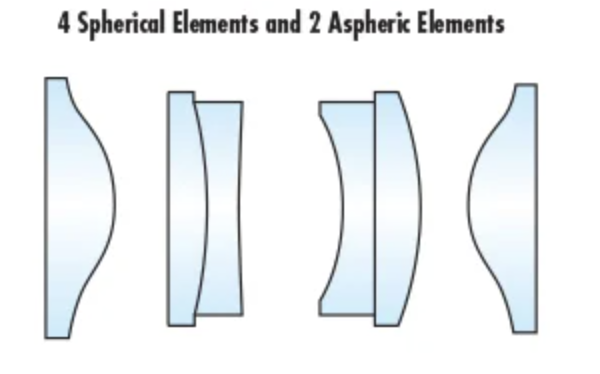
\includegraphics[scale=0.4]{lentilles_aspherique.png}
  \caption{Image de lentilles de forme anti-sphériques \textcolor{red}{(Source 3)}.}
  \label{lentilles_antisph}
\end{figure}

Une autre méthode pouvant diminuer les aberrations sphériques correspond à utiliser un système optique symétrique. Cette méthode consiste à placer deux lentilles de sorte que les aberrations créées par la première lentille soient corrigées par la deuxième lentille, souvent placée afin que les deux lentilles se miroitent.

En ce qui concerne la seconde aberration mentionnée, soit celle chromatique, celle-ci surviennent lorsque de la réfraction des rayons sur les lentilles. En effet, les différentes longueurs d'onde de la lumière, dû à leur diverse indice de réfraction, ne se focalisent pas au même point \textcolor{red}{(Source 2)}. Il existe deux types d'aberrations chromatiques, soit les longitudinales et les transversales. Dans le cas des caméras, les transversales sont les plus communes. Celles-ci résultent du décalage latéral des couleurs par rapport au point de focalisation \textcolor{red}{(Source 4)}. Une méthode de correction de ce type d'aberration est d'utiliser des verres comportant des caractéristiques qui compensent la réfraction des différentes longueurs d'onde telles que des lentilles achromatiques ou des lentilles à gradient d'indice.

% Source 1 : https://www.canon-europe.com/pro/infobank/aperture/

% Source 2 : https://www.edmundoptics.fr/knowledge-center/application-notes/imaging/how-aberrations-affect-machine-vision-lenses/

% Source 3 : https://www.edmundoptics.fr/knowledge-center/trending-in-optics/aspheric-lens-takeover/

% Source 4 : https://ressources.univ-lemans.fr/AccesLibre/UM/Pedago/physique/02/optiquecours/aberchro.html


\section{Conclusion}

\textcolor{red}{A FAIRE}

\clearpage

% \bibliographystyle{unsrtnat}
% \bibliography{My_Library}

\end{document}
